%  Created by Branden Stone on 2015-01-15.
%  Copyright (c) 2015 Branden Stone. All rights reserved.
%--------------------------------------------------------
\documentclass{article}


%---------------------------
% Packages
%---------------------------
\usepackage{amssymb, amsmath, latexsym, amsfonts, amsthm, mathrsfs} % Standard packages that are nice to have.
\usepackage{amsrefs} % Allows for easy referencing and citations.
\usepackage{verbatim} % Needed for \begin{comment} \end{comment}.
\usepackage[text={6in,9in},centering]{geometry} % Defines the dimensions of the text body.
\usepackage[colorlinks=true]{hyperref} % Allows for use of hyperlinks.
%\usepackage[doublespacing]{setspace} % Makes the document double spaced.
\usepackage[pdftex]{graphicx} % Allows for \includegraphics
\usepackage{enumerate} % Allows for easy modification of lists

\renewcommand{\arraystretch}{1.5}

%----------------------------
% Title and Author
%----------------------------

\title{Math 390 Homework 4}
\author{Due Wednesday, February 24}
\date{}


%----------------------------
% Main Document Body
%----------------------------

\begin{document}


%-------------------------------------------------------------
% Front Matter: This is where you can add a table of contents,
% preface, list of figures, ETC. for this template we will 
% only create a title and author name with `\maketitle'
%-------------------------------------------------------------

\maketitle

\setlength{\parindent}{0em} % Sets indentation of new paragraph
\setlength{\parskip}{1em} % Sets space between paragraphs

%-------------------------------------------------------------
% Document Body: Essentially this is where you place the 
% content of your document. To use this template, just delete
% all of the text between here and the Bibliography Section.
% Then type whatever you desire.
%-------------------------------------------------------------


Solutions should be written \LaTeX\ or Markdown and converted to a PDF. You are encouraged to work with others
on the assignment, but you should write up your own solutions independently. This means no copy pasting. You should
reference all of your sources, including your collaborators. 

\begin{enumerate}

\item Every morning a postman takes the bus to the post office. From there, he chooses a route to reach home as quickly as possible ({\bf NOT} ending at the post office). His route must include all of the streets in the map below. The map gives the number of minutes required to walk each block. Find the optimal route for the postman to travel (give the route and the total time that the route takes), and explain why the route is optimal.
\begin{center}
	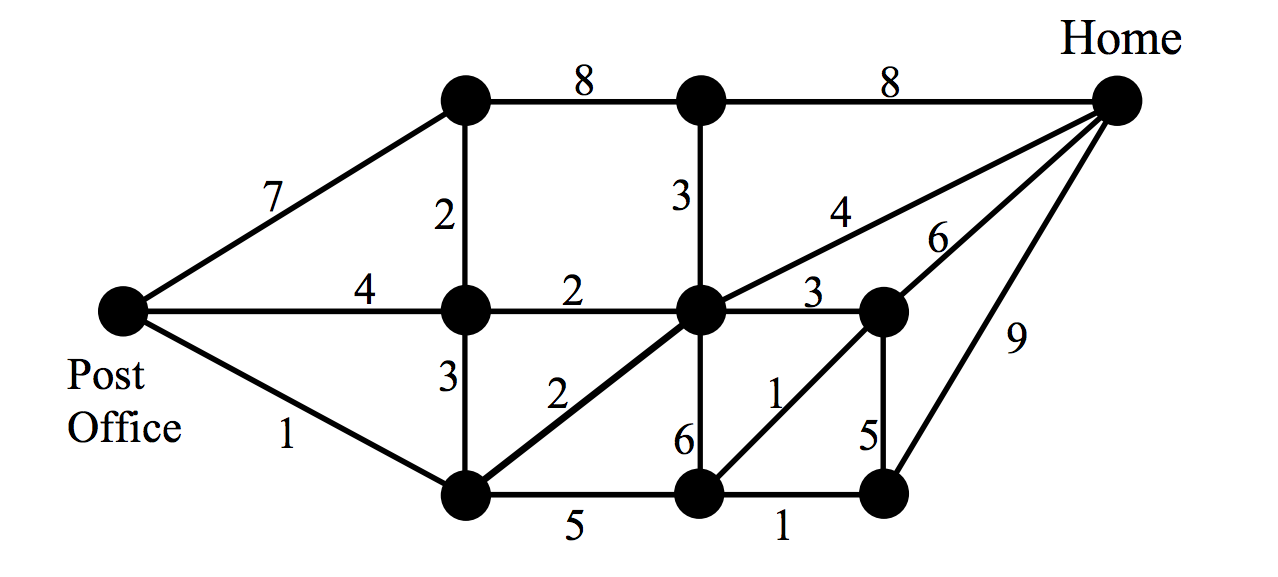
\includegraphics[width=.6\textwidth]{post-home2.png}
\end{center}

\item (Exercise 3.8/1.51) The {\bf complement} of a simple graph $G$ is a simple graph $\overline G$ with vertex set $V(G)$ where two vertices in $\overline G$ are adjacent if and only if they are not adjacent in $G$. A simple graph that is isomorphic to its complement is called {\bf self-complementary}.
\begin{enumerate}
	\item Prove that, if $G$ is self-complementary, then $G$ has $4k$ or $4k+1$ vertices, where $k$ is an integer.

	\item Find all self-complementary graphs with 4 and 5 vertices.

	\item Find a self-complementary graph with 8 vertices.
\end{enumerate}

\item First look up the definition of connectivity in your book. Now construct a 3-regular simple graph $G$ with connectivity $\kappa(G)=1$.

\item (Exercise 7.7/2.34)
\begin{enumerate}
	\item Let $G$ be a simple graph with $n$ vertices and $\displaystyle\binom{n-1} 2 +2$ edges. Use Ore's Theorem to prove that $G$ is Hamiltonian. 

	\item Find a simple non-Hamiltonian graph with $n$ vertices and $\displaystyle\binom{n-1} 2 + 1$ edges.
\end{enumerate}

\item (Exercise 10.3/3.17)
\begin{enumerate}
	\item Find the number of labeled trees on $n$ vertices in which vertex 1 is a leaf.

	\item Prove that if $n$ is large, then the probability that a given vertex of a tree with $n$ vertices is a leaf is approximately $e^{-1}$.
\end{enumerate}


\end{enumerate}





\end{document}